%%
%% Author: dariochinelli
%% 2021-03-11
%%

\section{Effetto Compton}

L'effetto Compton è, come l'effetto fotoelettrico, un fenomeno di interazione tra radiazione e materia, si tratta però di fotoni molto più energetici come i fotoni X.
È denominato scattering o diffusione poiché viene interpretato come un urto anelastico tra il fotone e l'elettrone per cui non vi è quindi assorbimento del fotone ed è questa la differenza fondamentale dall'effetto Compton.

\subsection{Esperimento di Compton}
\begin{figure}[h]
\centering
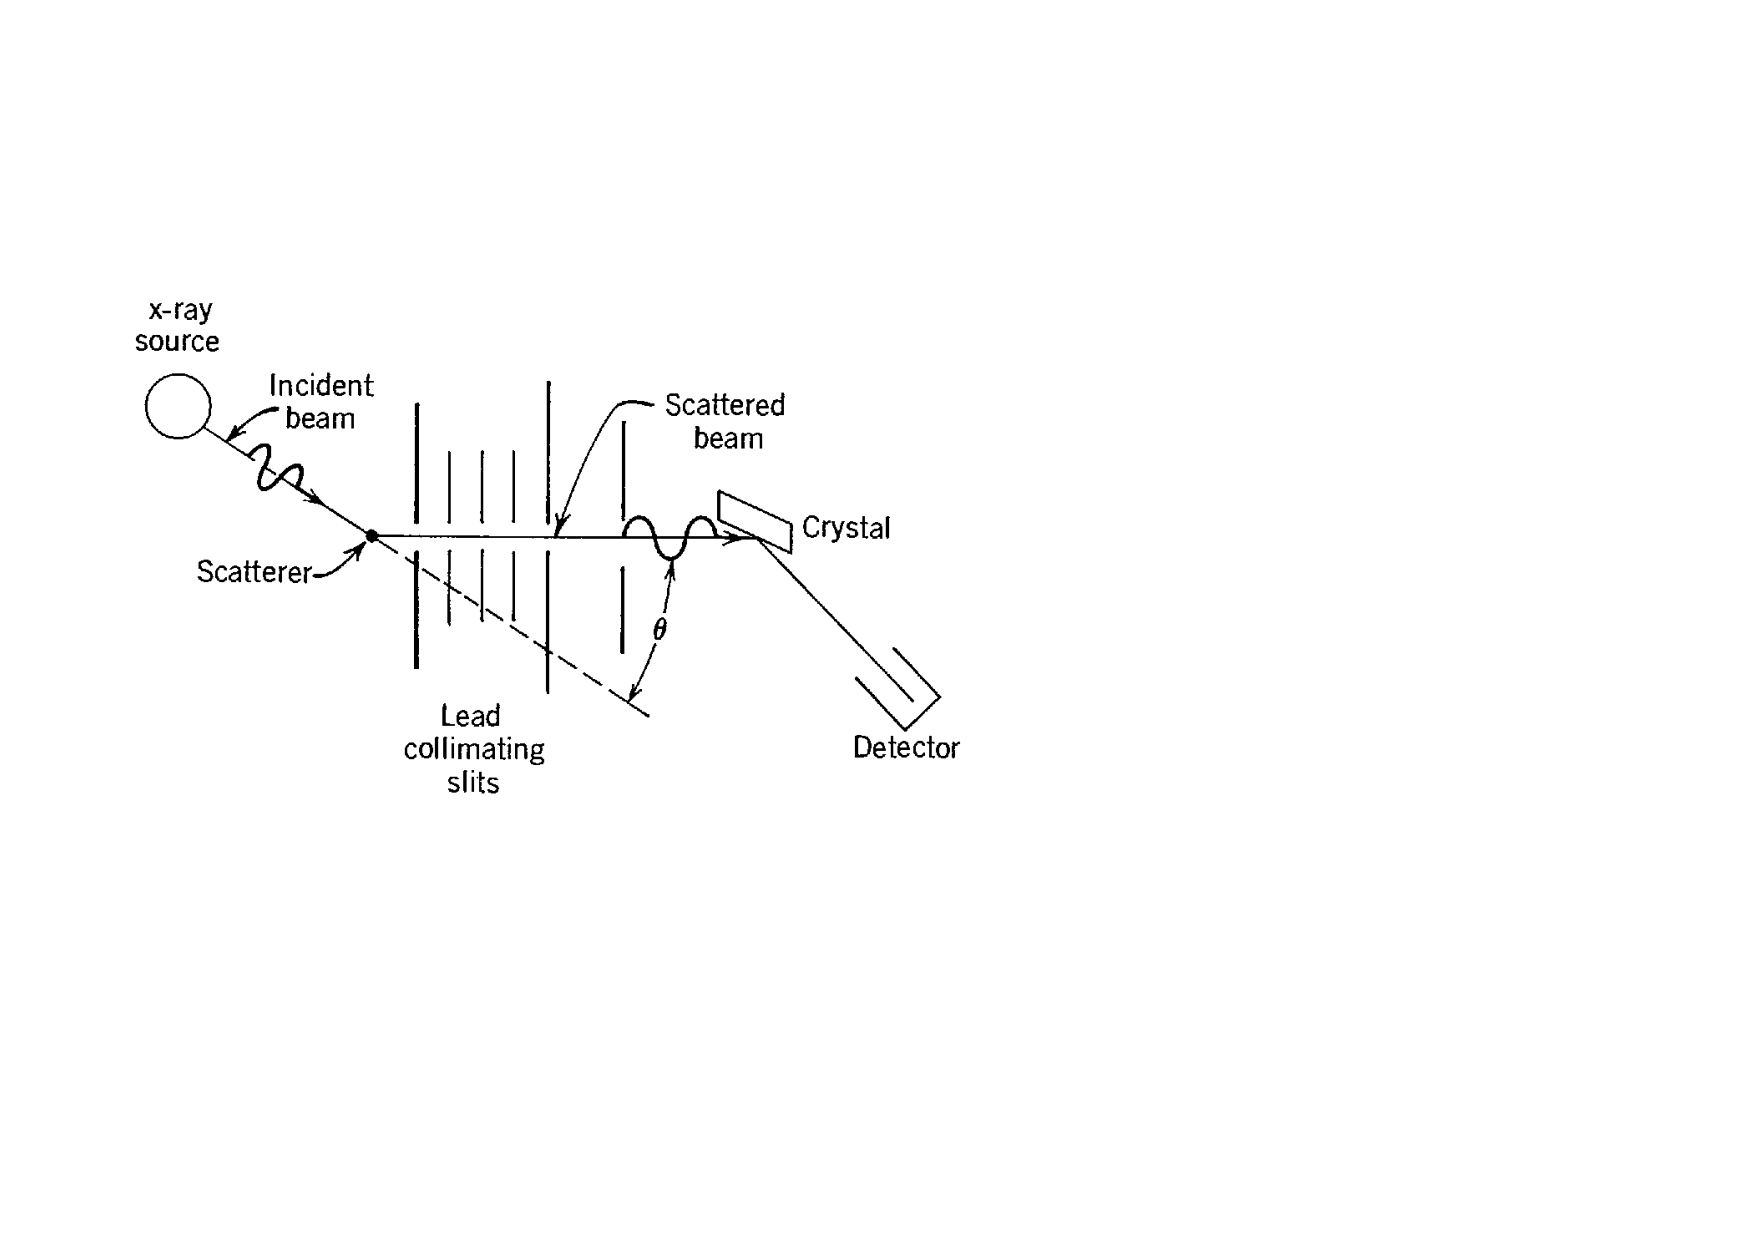
\includegraphics[scale=0.75]{/effettoCompton_setup}
\caption{Setup sperimentale dell'esperimento di Compton}
\end{figure}

Nell'esperimento del 1922, un fascio di fotoni X monocromatico, quindi una $\lambda = \SI{0.0709}{nm}$ molto precisa, viene fatto incidere su un target di carbonio, ed in seguito a questo viene diffusa radiazione X su tutto l'angolo solido.
Compton \textbf{misura l'intensità} della radiazione diffusa in funzione della lunghezza d'onda a diversi angoli di diffusione $\theta$.
Nell'apparato sperimentale vengono posti dei collimatori del fascio "slits" e l'apparato che consente di eseguire la misura: uno spettrometro di Bragg costituito da un cristallo e un detector, che vediamo in seguito.

Vediamo i risultati ottenuti da Compton in figura \ref{compton_results}.
Quando $\theta = 0$ si vede un picco di intensità, centrato sullo stesso valore di $\lambda$ del raggio incidente.
Se aumento l'angolo $\theta$ di fianco al primo picco ne compare un secondo ad una lunghezza d'onda maggiore rispetto al primo,
aumentando sempre di più l'angolo i due picchi si distinguono sempre meglio.
La presenza di questo secondo picco non è spiegabile con la fisica classica, solo il primo picco lo è.

\begin{figure}[h]
\centering
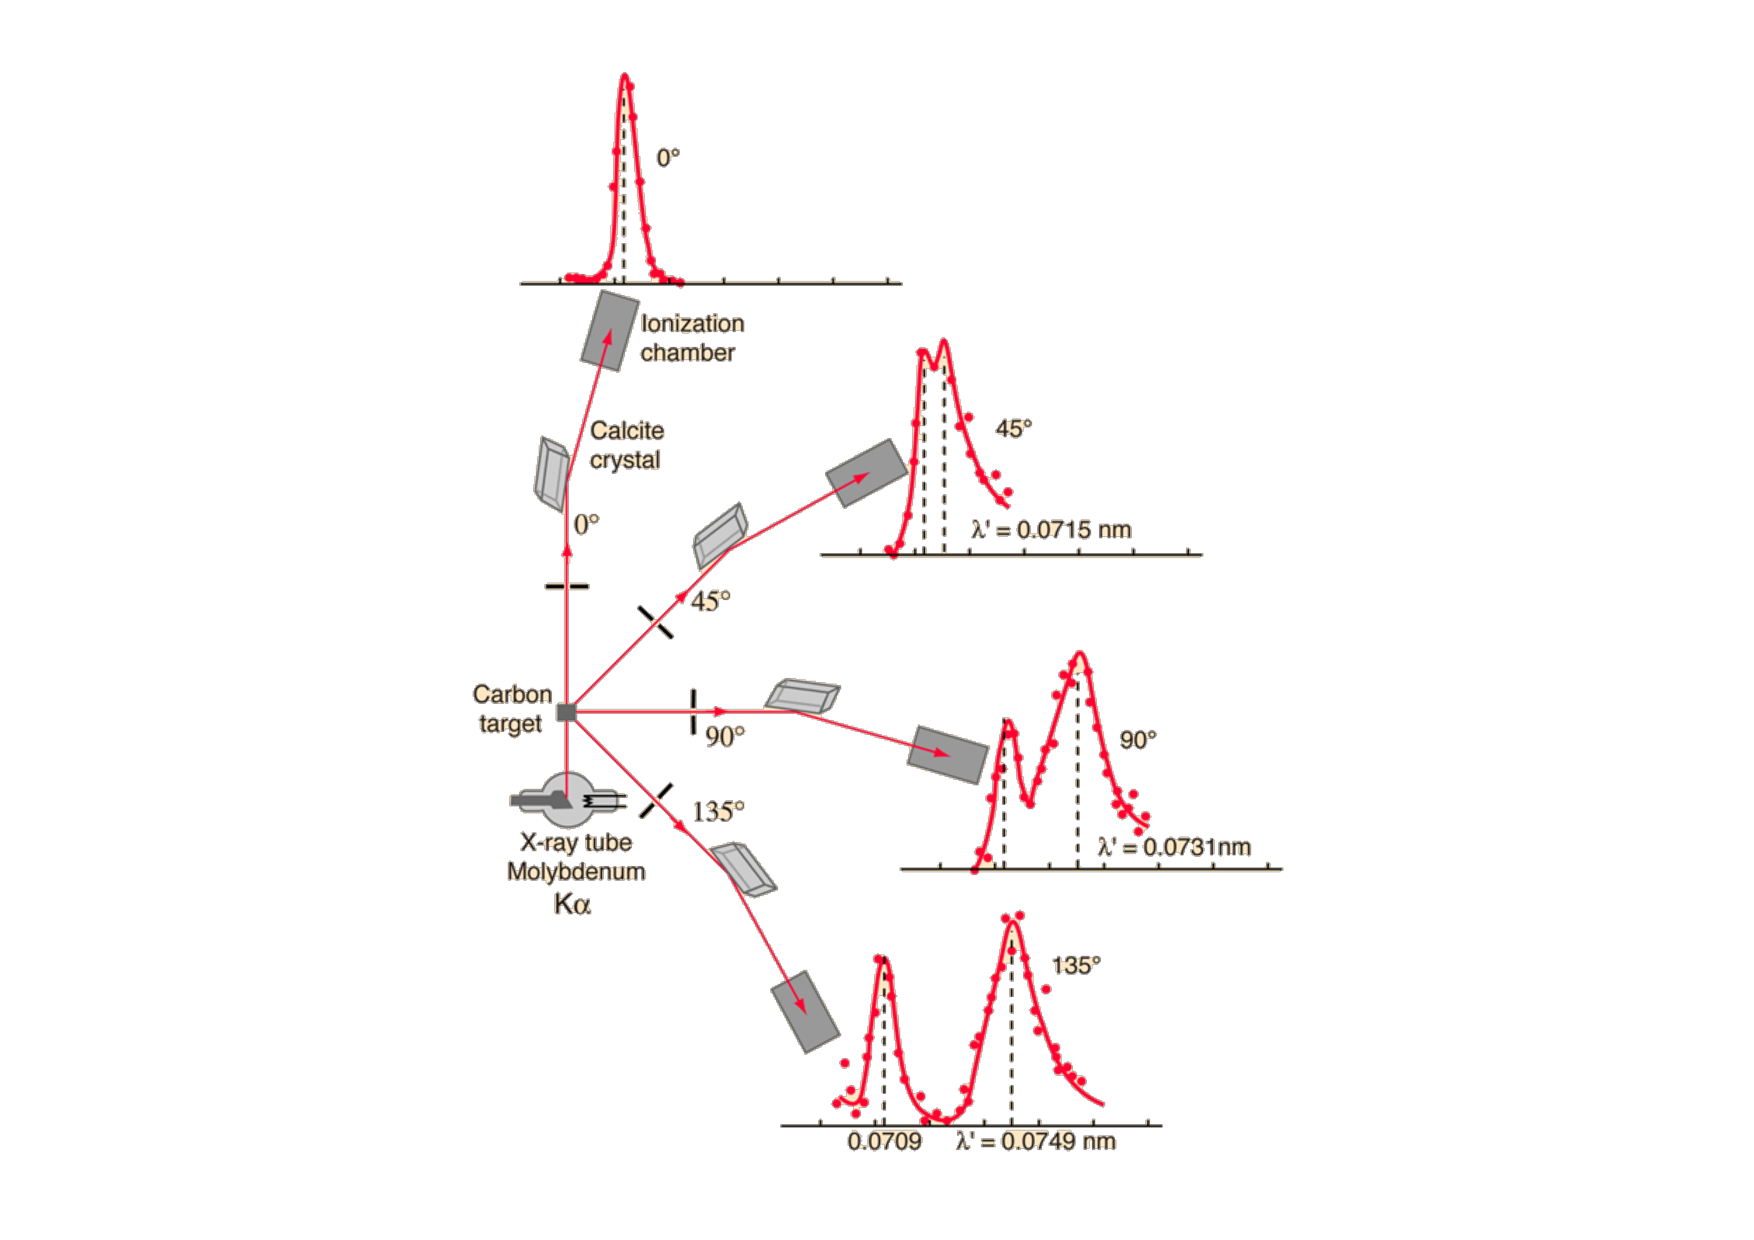
\includegraphics[scale=0.5]{/effettoCompton_risultati}
\caption{Risultati di Compton sulla misura dell'intensità della radiazione diffusa in funzione della lunghezza d'onda $\lambda$ a diversi angoli $\theta$}
\label{compton_results}
\end{figure}

\subsection{Spiegazione di Compton}

La spiegazione data da Compton (e Debye) è assumere che il fascio irraggiante X fosse composto da fotoni e che avvenisse un \textit{urto} tra un fotone e un elettrone \textit{libero} all'interno del target.
Quindi l'energia del fotone incidente $E$ iniziale verrà trasferita in parte all'elettrone, in seguito a ciò il fotone avrà energia finale minore e quindi lunghezza d'onda maggiore.
Nell'effetto Compton i fotoni non sono quindi assorbiti ma \textit{scatterati} e tali fotoni costituiranno il secondo picco rilevato nell'esperimento.
Definisco l'elettrone come \textit{libero} poiché il rapporto tra l'energia del fotone incidente e quella di estrazione dell'elettrone è molto grande, di conseguenza posso applicare alcune approssimazioni.

\begin{equation}
\begin{split}
E = \frac{ m_0 c^2}{\sqrt{1 - \frac{ v^2}{c^2 }} } & \quad \mbox{energia di una particella relativistica con massa} \\
E = h \nu & \quad \mbox{energia del fotone, che ha massa nulla} \\ \\
E^2 = c^2 p^2 + (m_0 c^2)^2 & \quad \mbox{per il fotone il secondo termine è zero} \\
p = \frac{ E}{c } = \frac{ h \nu}{c } = \frac{ h}{ \lambda} & \quad \mbox{quantità di moto del fotone} \quad \mbox{dove uso} \quad \lambda \nu = c
\end{split}
\end{equation}

Studiamo il processo di interazione uguagliando il momento totale prima e dopo l'interazione e l'energia totale prima e dopo la collisione.
Indico con $E_0, p_0$ l'energia e il momento del fotone incidente e con $\lambda$ la sua lunghezza d'onda, considero l'elettone inizialmente fermo.
Dopo la collisione indico con $E_1, p_1$ l'energia e il momento del fotone diffuso e con $\lambda'$ la sua lunghezza d'onda; 
indico con $K, p$ l'energia ed il momento dell'elettrone dopo l'urto;
indico inoltre con $\theta$ l'angolo di diffusione del fotone e con $\phi$ l'angolo di diffusione dell'elettrone.
Considerare inoltre che, al contrario del fotone, l'elettrone ha massa e quindi energia a riposo non nulla pari a $m_{0,e}c^2$.

\begin{figure}[h]
\centering
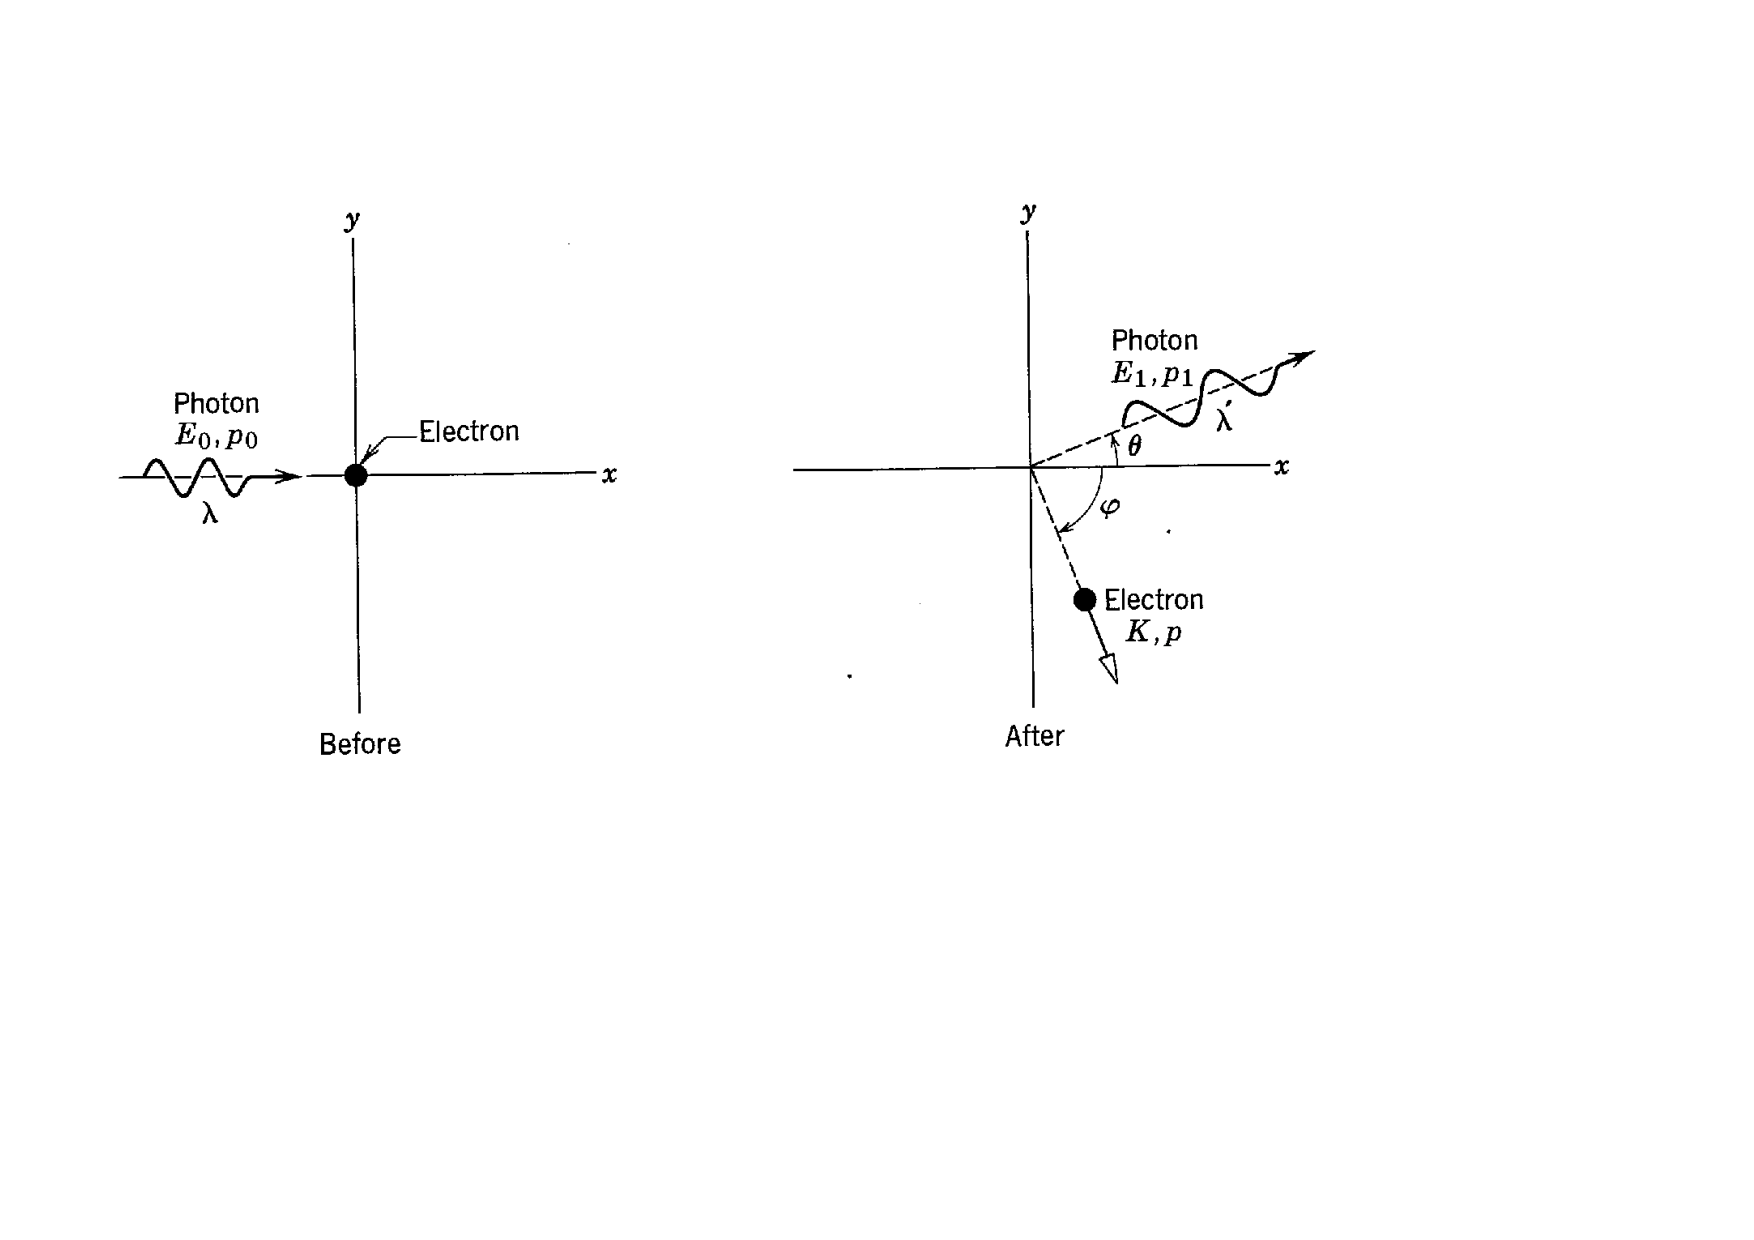
\includegraphics[scale=0.6]{/effettoCompton_schema_interazione}
\caption{ Effetto Compton. Un fotone di lunghezza d'onda $\lambda$ incide su un elettrone a riposo. 
Nella collisione il fotone è scatterato di un angolo $\theta$ con lunghezza d'onda maggiore $\lambda '$, 
mentre l'elettrone si allontana con angolo $\varphi$ }
\end{figure}

Applichiamo la conservazione del momento angolare
\begin{equation}
\begin{split}
\mbox{lungo x} \quad & p_0 = p_1 \cos\theta + p \cos\varphi \\
\mbox{lungo y} \quad & p_1 \sin\theta = p \sin\varphi \\ \\
& (p_0 - p_1 \cos\theta)^2 = p^2 \cos^2\varphi \\
& p_1^2 \sin^2\theta = p^2 \sin^2\varphi \\ \\
\mbox{ottengo} \quad & p_0^2 + p_1^2 = 2 p_0 p_1 \cos\theta = p^2
\end{split}
\end{equation}

Applichiamo la conservazione dell'energia
\begin{equation}
\begin{split}
& E_0 + m_{0,e} c^2 = E_1 + K + m_{0,e} c^2 \\
& E_0 - E_1 = K \\ \\
\mbox{utilizzando} \quad & p =\frac{ E}{c } \\
\mbox{ottengo} \quad & c (p_0 - p_1) = K 
\end{split}
\end{equation}

Dalla relazione di mass shell relativistica applicata all'elettrone ottengo
\begin{equation}
\begin{split}
& E^2 = c^2 p^2 + (m_{0,e} c^2)^2 \\
& (K + m_{0,e} c^2)^2 = c^2 p^2 + (m_{0,e} c^2)^2 \\
& K^2 + 2 K m_{0,e} c^2 = c^2 p^2 \\
& \frac{ K^2}{c^2 } + 2Km_{0,e} = p^2
\end{split}
\end{equation}

In quest'ultima relazione sostituisco ora $p$ e $K$ dai risultati ottenuti in precedenza e trovo
\begin{equation}
\begin{split}
& (p_0 - p_1)^2 + 2m_{0,e} c (p_0 - p_1) = p_0^2 + p_1^2 - 2p_0 p_1 \cos\theta \\
& m_{0,e} c (p_0 - p_1) = p_0 p_1 (1 - \cos\theta) \\ \\
& \frac{ 1}{p_0 } - \frac{ 1}{p_1 } = \frac{ 1}{m_{0,e} c } (1 - \cos\theta)
\end{split}
\end{equation}

Moltiplicando per la costante di Planck $h$ ed utilizzando la formula $c = \lambda \nu$ si ottiene
\begin{equation}
\begin{split}
& \Delta \lambda = \lambda' - \lambda = \lambda_c (1 - \cos \theta) \\
& \lambda_c = \frac{ h}{m_{0,e} c } = \SI{2.43e-12}{m} = \SI{0.0000243}{nm} = \SI{2.43}{pm} = \SI{0.0243}{\AA}
\end{split}
\end{equation}
$\Delta \lambda$ definisce la distanza tra i due picchi visti nel grafico dei risultati dell'esperimento di Compton, inoltre la costante $\lambda_c$ è detta \textit{lunghezza d'onda di Compton}. \\
Quindi lo shift di Compton dipende \underline{solo} da $\theta$, per cui il valore minimo $\Delta \lambda = 0$ si ha per $\theta = 0$ ed il valore massimo $\Delta \lambda = \frac{ 2 h }{m_{0,e} c }$ per $\theta = \pi$.

\begin{figure}[h]
\centering
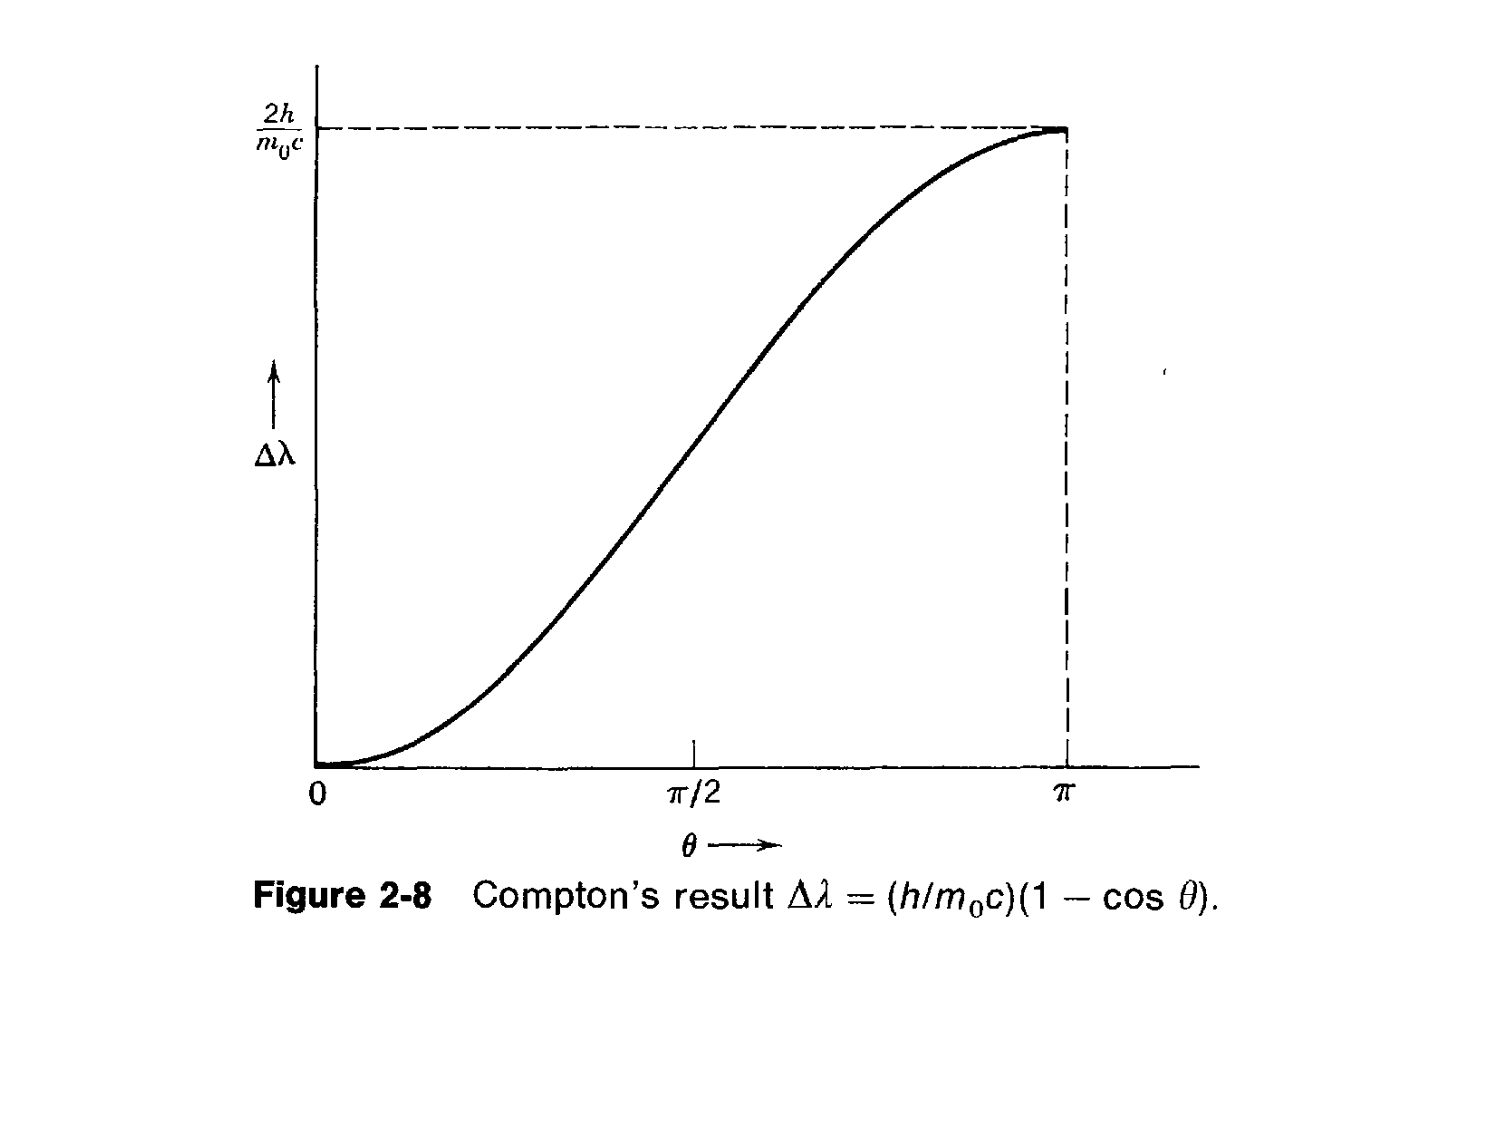
\includegraphics[scale=0.5]{/compton_deltalambda}
\caption{Andamento di $\Delta\lambda$ in funzione dell'angolo $\theta$}
\end{figure}

\textbf{NB:} Nell'esperimento di Compton ho due processi di interazione fra radiazione e materia: alcuni fotoni sono diffusi da elettroni che considero liberi e che vengono poi espulsi dal materiale, altri fotoni vengono diffusi da elettroni che rimangono legati al nucleo per cui non vi è una variazione della lunghezza d'onda dei fotoni, questo secondo processo prende il nome di scattering di Rayleigh (o scattering di Thompson).
Se la radiazione incidente fosse nel visibile o nelle onde radio, la lunghezza d'onda sarebbe talmente grande rispetto allo shift che non si potrebbe osservare tale fenomeno.

